

Earthquakes, hurricanes, and other large-scale disasters cause widespread damage
to physical infrastructure, and Internet routing infrastructure is no exception.
In 2006, an earthquake in Taiwan severed six of seven 
undersea cables connecting North and Southeast Asia with each other and North 
America. 
Regional disasters like these have the potential to generate substantial 
correlated failures when multiple links disconnect and entire Exchange Points
go dark.

\eat{
The United States government defines {\it critical infrastructure} as ``systems
and assets, whether physical or virtual, so vital to the United States that the
incapacity or destruction of such systems and assets would have a debilitation
impact on security, national economic security, national public health or
safety, or any combination of those matters''~\cite{patriotact}. Internet
connectivity, a fundamental requirement for modern communication, is
undoubtedly such a system.  Businesses~\cite{something?} and
governments~\cite{cyberspacepolicy} hence value the physical security of
Internet infrastructure to disaster.
}

In this paper, we explore the impact of regional disasters on Internet
connectivity using a new modeling technique, geodesic failure regionalization.
While previous work in Internet resilience focused primarily on logical
connectivity, we map peering relationships to one or more geographic regions
where peering takes place.  We approximate geographic regions by generating a
polyhedron whose faces represent a contiguous area suceptible to disaster.  We
then use publicly available peering datasets~\cite{brice, peeringdb},
traceroutes, and DNS and commercial geolocation techniques to map locations
where networks peer (exchange points or private peering facilities) to faces on
the polyhedron.  We use this model to simulate the impact of regional failures,
\ie{} the removal of one or more faces, and investigate the following issues:

\noindent{\bf Regional Peering Redundancy.} How many regions do networks
typically peer in? How does it scale with the degree of the network?

\noindent{\bf Quantifying Resilience.} Can we quantify the resiliance of a
network to failure terms of it's number of peers, global footprint, and number
of regions it peers in?

\noindent{\bf Identifying Worst-Case Scenarios.} Are there bottlenecks in the
physical connectivity graph? How badly could the network partition in a
worst-case regional disaster?

We are not the first to evaluate Internet resilience to
failures~\cite{michigan, measuringresilience, resilience-under-BGP,
resilience-complex-networks}.  Our contribution is to consider the impact of
physical disaster on the observed connectivity map.  Previous work focused on
the impact of severing logical links, that is, declaring that two networks had
been entirely disconnected.  This type of model cannot capture the network
impact of physical disaster.  For example, it is highly unlikely that two Tier
1 networks would be partitioned in any single event.  These networks have
global footprints and connect at multiple physical locations.
  On the other hand, disconnecting logical links
one by one ignores the physical reality that any disaster that strikes a link
in shared infrastructure such as an IXP is likely to impact a large number of
links.  In this case, modeling failure of a single logical link is an
underestimate.  We argue that focusing on physical connectivity is the best way to
develop models of the impact of physical disaster. 
 
\begin{figure*}[htb]
\centering
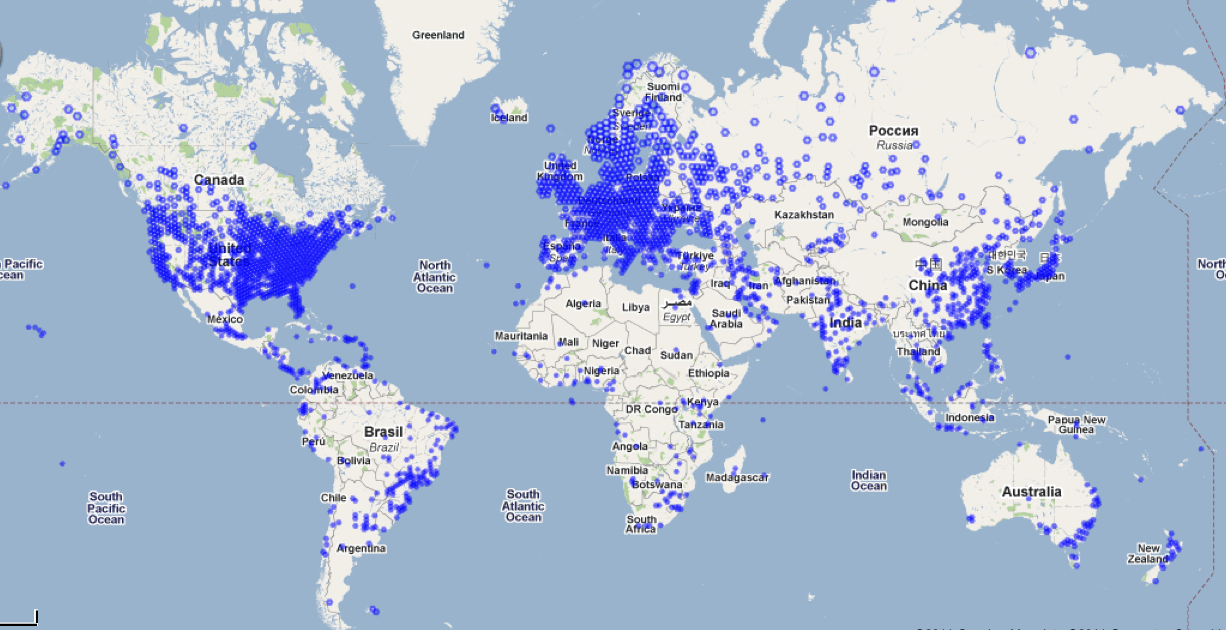
\includegraphics[width=6in]{world_map.jpg}
\caption[]{\label{fig:worldmap} \shaddi{Fig porfavor} Illustration of geodesic cells, or failure regions, on the world map. Shaded cells are regions which include two or more networks peering. The average cell includes \kristin{n} ASes involved in \kristin{m} peering relationships.} 
\end{figure*}

Before we move forward, we clarify the scope of our goals.  Evaluations of
AS-level connectivity graphs show that traceroute-based topologies like those
that we rely upon are in many ways incomplete~\cite{walter}.  For instance,
policy compliant routing ensures that measurements made with only limited
vantage points cannot observe peering relationships between networks where
neither network contains a measurement vantage point.  Further, `backup links',
which are provisioned for the case of failure but otherwise unused, cannot be
observed since no traffic flows across these links when the primary links are
available.  These and other impediments mean that any analysis over
measurement-based graphs may be missing critical information.  Thus, the
results of our study should not be considered hard and fast projections of
Internet connectivity.  Instead, we aim only to provide {\it estimates} and
{\it bounds} on the impact of regional disaster on Internet routing.

Our results estimate that \justine{\ldots}

The remainder of the paper is organized as follows. In \S\ref{sec:connectivity_model}, we describe our model of global connectivity.
In \S\ref{sec:quant_connect}, we provide basic observations of our data quantifying how often transit networks peer and in how many different geographic regions.
Completing our analysis, we describe our failure analysis in \S\ref{sec:failures}.
Finally, we describe related work in  \S\ref{sec:related_work} and conclude in \S\ref{sec:conclusion}.
